%%%%%%%%%%%%%%%%%%%%%%%%%%%%%%%%%%%%%%%%%
% The Legrand Orange Book
% LaTeX Template
% Version 3.1 (February 18, 2022)
%
% This template originates from:
% https://www.LaTeXTemplates.com
%
% Authors:
% Vel (vel@latextemplates.com)
% Mathias Legrand (legrand.mathias@gmail.com)
%
% License:
% CC BY-NC-SA 4.0 (https://creativecommons.org/licenses/by-nc-sa/4.0/)
%
% Compiling this template:
% This template uses biber for its bibliography and makeindex for its index.
% When you first open the template, compile it from the command line with the 
% commands below to make sure your LaTeX distribution is configured correctly:
%
% 1) pdflatex main
% 2) makeindex main.idx -s indexstyle.ist
% 3) biber main
% 4) pdflatex main x 2
%
% After this, when you wish to update the bibliography/index use the appropriate
% command above and make sure to compile with pdflatex several times 
% afterwards to propagate your changes to the document.
%
%%%%%%%%%%%%%%%%%%%%%%%%%%%%%%%%%%%%%%%%%

%----------------------------------------------------------------------------------------
%	PACKAGES AND OTHER DOCUMENT CONFIGURATIONS
%----------------------------------------------------------------------------------------

\documentclass[
	12pt, % Default font size, select one of 10pt, 11pt or 12pt
	fleqn, % Left align equations
	a4paper, % Paper size, use either 'a4paper' for A4 size or 'letterpaper' for US letter size
	%oneside, % Uncomment for oneside mode, this doesn't start new chapters and parts on odd pages (adding an empty page if required), this mode is more suitable if the book is to be read on a screen instead of printed
]{LegrandOrangeBook}

% Book information for PDF metadata, remove/comment this block if not required 
\hypersetup{
	pdftitle={A NEAT Inspired GEP Algorithm}, % Title field
	pdfauthor={Louis John Hassett, Duncan Anthony Coulter, Daniel Ogwok}, % Author field
	pdfsubject={Evolutionary Computing, Neural Networks}, % Subject field
	pdfkeywords={NEAT, GEP}, % Keywords
	pdfcreator={LaTeX}, % Content creator field
}

\addbibresource{sample.bib} % Bibliography file

\definecolor{ocre}{RGB}{128, 0, 0} % Define the color used for highlighting throughout the book

\chapterimage{} % Chapter heading image
\chapterspaceabove{6.5cm} % Default whitespace from the top of the page to the chapter title on chapter pages
\chapterspacebelow{6.75cm} % Default amount of vertical whitespace from the top margin to the start of the text on chapter pages

%----------------------------------------------------------------------------------------
\usepackage{epigraph}
\usepackage[autostyle=true]{csquotes} % Required to generate language-dependent quotes in the bibliography

\linespread{1.5}
\begin{document}

%----------------------------------------------------------------------------------------
%	TITLE PAGE
%----------------------------------------------------------------------------------------

\titlepage % Output the title page
	{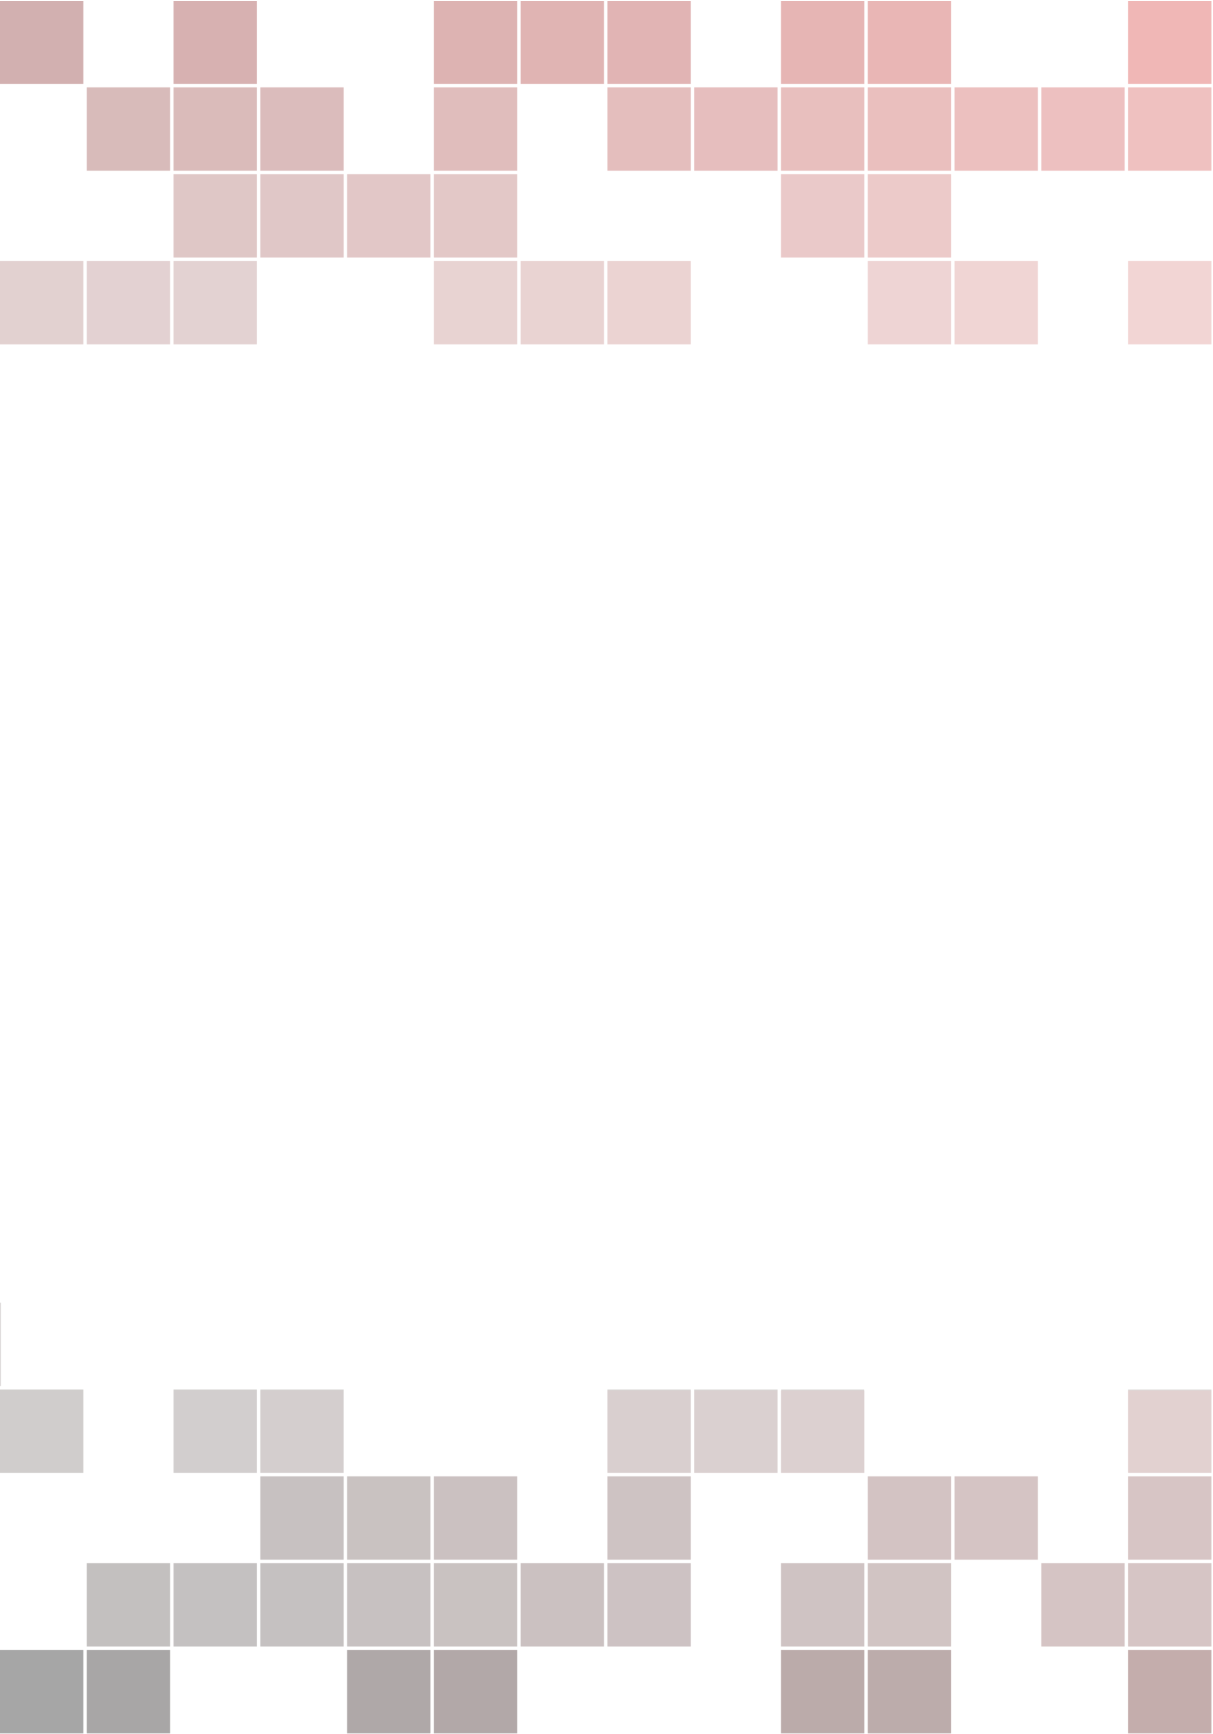
\includegraphics[width=\paperwidth]{background.pdf}} % Code to output the background image, which should be the same dimensions as the paper to fill the page entirely; leave empty for no background image
	{ % Title(s) and author(s)
		\centering\sffamily % Font styling
		{\LARGE \href{https://www.uj.ac.za/}{University of Johannesburg}\par} % Subtitle
		\vspace{16pt}
		{\large Masters Dissertation\par} % Subtitle
		\vspace{16pt} % Vertical whitespace
		{\Huge\bfseries A NEAT Inspired GEP Algorithm\par} % Book title
		\vspace{16pt} % Vertical whitespace
		% {\huge\bfseries Louis John Hassett\par} % Author name

		\begin{minipage}[t]{0.4\textwidth}
		\begin{flushleft} \large
		\emph{Author:}\\
		\href{http://www.johnsmith.com}{Louis John Hassett} % Author name - remove the \href bracket to remove the link
		\end{flushleft}
		\end{minipage}
		\begin{minipage}[t]{0.4\textwidth}
		\begin{flushright} \large
		\emph{Supervisor:} \\
		\href{http://www.jamessmith.com}{Prof. Duncan A. Coulter} \\ % Supervisor name - remove the \href bracket to remove the link  
		\emph{Co-supervisor:} \\
		\href{http://www.jamessmith.com}{Daniel Ogwok}
		\end{flushright}
		\end{minipage}\\[1cm]

		\large \textit{A dissertation submitted in fulfillment of the requirements\\ for the degree of Master in Computer Science}\\[0.3cm] % University requirement text
		\textit{in the}\\[0.4cm]
		\href{https://adam.uj.ac.za/academy/}{Faculty of Science\\Academy of Computer Science and Software Engineering}\\ % Research group name and department name
	}


%----------------------------------------------------------------------------------------
%	COPYRIGHT PAGE
%----------------------------------------------------------------------------------------

\thispagestyle{empty} % Suppress headers and footers on this page

\noindent\enquote{\itshape It is not the strongest of the species that survives, nor the most intelligent that survives. It is the one that is most adaptable to change. In the struggle for survival, the fittest win out at the expense of their rivals because they succeed in adapting themselves best to their environment.}\bigbreak

\hfill Charles Darwin


~\vfill % Push the text down to the bottom of the page

\noindent \textbf{Acknowledgements} \\
I would like to sincerely thank my supervisor, Prof Coulter, for his guidance and support throughout this research. His expertise and feedback were invaluable. 


%----------------------------------------------------------------------------------------
%	TABLE OF CONTENTS
%----------------------------------------------------------------------------------------

\pagestyle{empty} % Disable headers and footers for the following pages

\tableofcontents % Output the table of contents

\listoffigures % Output the list of figures, comment or remove this command if not required

\listoftables % Output the list of tables, comment or remove this command if not required

\pagestyle{fancy} % Enable default headers and footers again

\cleardoublepage % Start the following content on a new page

%----------------------------------------------------------------------------------------
%	PART
%----------------------------------------------------------------------------------------

% \part{Part One Title}

%----------------------------------------------------------------------------------------
%	SECTIONING EXAMPLES CHAPTER
%----------------------------------------------------------------------------------------
\chapterimage{} % Chapter heading image
\chapterspaceabove{6.75cm} % Whitespace from the top of the page to the chapter title on chapter pages
\chapterspacebelow{7.25cm} % Amount of vertical whitespace from the top margin to the start of the text on chapter pages

%------------------------------------------------
\chapterimage{} % Chapter heading image
\chapterspaceabove{6.75cm} % Whitespace from the top of the page to the chapter title on chapter pages
\chapterspacebelow{7.25cm} % Amount of vertical whitespace from the top margin to the start of the text on chapter pages
\chapter{Introduction}\index{chapter:introduction}
\section{Background}
The theory of evolution by natural selection, first introduced by Charles Darwin, has profoundly influenced our understanding of the life and adaption in the natural world. Darwin's insight that species evolved over generations through the survival and reproduction of individuals with advantageous traits has not only shaped the biological sciences, but has also inspired computational models that emulate these adaptive processes (\cite{basicsOfEvolutionaryComputing}). Over millions of years, evolution has given rise to complex biological systems, among which the human brain stands as one of the most intricate. Composed of billions of neurons, the brain processes information through electrochemical signaling across complex interconnected networks, enabling perception, reasoning, and decision-making (\cite{engelbrecht2007computational}). These biological mechanisms have served as a blueprint for the development of artificial intelligent systems, particular in the field of evolutionary computation and neural networks.

\parbreak

\noindent In computer science, evolutionary algorithms simulate the process of natural selection to solve complex optimisation problems. These algorithms operate on populations of candidate solutions, applying genetic operators such as mutation, crossover, and selection to iteratively improve the problem's solution. In conjunction to the expanding field of evolutionary computing, artificial neural networks (ANNs) which are inspired by the structure and function of biological neurons have become foundational in machine learning. These networks consist of interconnected nodes that process information in layers, enabling machines to learn from data and perform tasks such as classification, prediction, and control (\cite{russell2016artificial}). The intersection of evolutionary algorithms and neural networks has given rise to the field of neuroevolution, which seeks to evolve both the structure and parameters of neural networks using evolutionary principles.

\parbreak

\noindent Among the many algorithms developed within the field of evolutionary computing and neuroevolution, Gene Expression Programming (GEP) and the NeuroEvolution of Augmenting Topologies (NEAT) stand out due to their unique and complementary approaches to evolving computational structures. Gene Expression Programming (GEP) is an evolutionary algorithm that evolves computer programs or symbolic expressions. It represents solutions as linear chromosomes, which are then expressed as expression trees through an effective genotype-to-phenotype mapping scheme. This approach allows the evolution of tree-like structures in a more robust and flexible manner than traditional genetic programming techniques (\cite{ferreira2006gene}). NEAT, in contrast, focuses on evolving the topology and weights of neural networks. It introduces several key innovations, including historical markings (innovation numbers) to track structural changes, speciation to preserve diversity within the population, and incremental growth of network complexity to efficiently explore the search space. These features enable NEAT to evolve increasingly sophisticated neural architectures over time (\cite{stanley2002evolving}).

\parbreak

\noindent This dissertation introduces a novel hybrid algorithm, GEP-NEAT, which seeks to combine the structural expressiveness of GEP with the adaptive topology evolution of NEAT. The motivation for developing GEP-NEAT arises from specific limitations observed in both NEAT and GEP-based neural network approaches. While NEAT has demonstrated success in evolving neural network topologies, it suffers from computational inefficiencies, particularly due to the overhead introduced by topological sorting during network evaluation which becomes increasingly problematic as networks grow in complexity. On the other hand, GEP-NN, an approach that applies GEP to evolve neural networks, offers promising alternative by representing neural structures as expression trees, but it remains relatively underexplored in the literature and lacks the methodological maturity and empirical validation seen in other neuroevolutionary techniques. GEP-NEAT is proposed a response to these challenges, aiming to combine the structural flexibility of GEP with the evolutionary dynamics of NEAT. At the heart of GEP-NEAT is a new representation scheme in which innovation numbers are encoded as sub-tree configurations. This approach allows for a more expressive and hierarchical encoding of neural structures, facilitating the reuse of functional subcomponents and promoting the emergence of modular architectures. By integrating GEP's symbolic representation with NEAT's evolutionary dynamics, GEP-NEAT aims to provide a more powerful and flexible tool for evolving neural networks.

\section{Structure}
This dissertation begins with this introductory chapter, which outlines the research motivation, and key research questions. It also highlights the academic contributions of the work, including publications that have emerged from the research process. Following the introduction, a dedicated chapter is presented on the research methodology, which adopts a design science approach. This chapter details the methodological framework used to guide the development, implementation, and evaluation of the proposed algorithm.

\parbreak

\noindent The core of the dissertation presents a comprehensive literature review, divided into three chapters. The first of these explores the foundations of evolutionary computing, providing context for the broader field in which the work is situated. The focuses on neuroevolution, examining how evolutionary algorithms have been applied to the development of neural networks. The third chapter delves into gene expression programming, detailing its mechanisms, advantages, and relevance to the proposed approach.

\parbreak

\noindent After establishing the theoretical foundation, the dissertation introduces the GEP-NEAT algorithm in detail. This chapter covers the theoretical underpinnings of the algorithm, its practical implementation, and the experimental setup used to evaluate its performance. The results of these experiments are then presented and analysed, with a focus on assessing the algorithm's effectiveness, efficiency, and potential advantages over existing methods. The final chapter concludes the dissertation by summarising the key findings, discussing their implications, and outlining directions for future research.

\section{Research Questions}
The development of algorithms that evolve neural network architectures remains a dynamic and evolving area of research. While various approaches have been proposed to automate the design of neural networks through evolutionary computation, several open questions persist regarding the efficiency, expressiveness, and adaptability of these methods. This dissertation is driven by a set of research questions that aim to explore and address specific limitations in existing neuroevolutionary techniques, particularly GEP and NEAT.

\parbreak

\noindent The first research question investigates the structural limitations of current gene expression programming when applied to neural networks. Traditional neural networks typically include architectural features such as bias nodes and non-linear activation functions, which are essential for enhancing representational capacity. However, many implementations of gene expression programming for neural networks do not incorporate these features. This leads to the first question:

\begin{researchquestion}{1}
    \textit{How can gene expression programming be extended to evolve neural networks that closely resemble traditional architectures, including the incorporation of bias nodes and activation functions?}
\end{researchquestion}

\parbreak

\noindent The second question addresses a known computational bottleneck in topology-based neuroevolutionary algorithms. Specifically, algorithms that evolve network structures often rely on topological sorting to ensure valid signal flow during evaluation. While effective, this process can become increasingly inefficient as networks grow in size and complexity. This raises the question:

\begin{researchquestion}{2}
    \textit{Can the computational inefficiencies associated with topological sorting in neural network evaluation be mitigated through alternative representations or evaluation strategies?}
\end{researchquestion}

\parbreak

\noindent A third area of inquiry concerns the role of innovation numbers in NEAT. Traditionally, innovation numbers are used to track structural changes and align genomes during crossover, however, this usage is largely historical and does not contribute directly to the functional behavior of the algorithm. This lead to the question:

\begin{researchquestion}{3}
    \textit{Is it possible to redefine innovation numbers in NEAT to represent meaningful and reusable structural components?}
\end{researchquestion}

\parbreak

\noindent Building on this idea, the fourth question explores the practical implications of such a redefinition. If innovation numbers can be used to encode modular structures, it is important to understand how this can be leverages to improve algorithmic performance. Thus, the next question is:

\begin{researchquestion}{4}
    \textit{Provided that innovation numbers are redefined as reusable structural components, how can this representation be exploited to improve the performance, modularity, or evolutionary dynamics of the algorithm?}
\end{researchquestion}

\parbreak

\noindent The fifth question considers the broader hypothesis that combining distinct evolutionary strategies may lead to improved outcomes. Specifically, it examines whether integrating symbolic expression-based representations (GEP) with topological representations (NEAT) can result in a more effecting approach to evolving neural networks. This gives rise to the question:

\begin{researchquestion}{5}
    \textit{Does the integration of symbolic-based representations (GEP) with topology-evolving strategies (NEAT) result in improved performance, scalability, or expressiveness compared to using either approach in isolation?}
\end{researchquestion}

\parbreak

\noindent Finally, the sixth question addresses a practical limitation in many symbolic neuroevolutionary systems, that is, the difficulty of evolving neural networks with multiple outputs. Many real-world tasks require networks to produce more than one output simultaneously, yet existing representations often struggle to accommodate this. This leads to the final question:

\begin{researchquestion}{6}
    \textit{How can expression trees be adapted to support the evolution of neural networks with multiple outputs, and what are the implications for multi-output learning tasks?}
\end{researchquestion}

\parbreak

\noindent Together, these research questions form the foundation of this dissertation. They aim to explore the theoretical and practical challenges of evolving neural networks using symbolic and structural representations, and to investigate whether new approaches can overcome the limitations in existing methods.

\section{Publications Resulting from this Work}\index{sec:publication\_from\_resulting\_work}
A peer-reviewed conference paper derived from this research was published in the proceedings of the \textbf{8th International Conference on Information Science and Systems (ICISS 2025)}. As an established forum in its eight iteration, ICISS maintains rigorous academic standards through its double-blind peer review process, where both author and reviewer identities are concealed to remove bias and ensure impartial evaluation based solely on scholarly merit. The conference brings together leading researchers across ten interdisciplinary tracks spanning artificial intelligence, data science, and information systems.

\parbreak

\noindent The accepted paper, which contributes to the Machine Learning and Artificial Intelligence track, presents the algorithm GEP-NEAT with its innovation number novelty, showcasing the ability to solve the XOR and Cart Pole problem effectively. ICISS 2025 facilitated valuable scholarly exchange through keynote presentations by field leaders, technical workshops, and interdisciplinary discussion bridging academic and real-world application. The conference proceedings are to be published into \textbf{Communications in Computer and Information Sicence (Electronic ISSN: 1865-0937 \& Print ISSN: 1865-0929)} as a proceedings book volume and indexed by EI Compendex, Scopus, INSPEC, SCImago and other databases.

\chapterimage{} % Chapter heading image
\chapterspaceabove{6.75cm} % Whitespace from the top of the page to the chapter title on chapter pages
\chapterspacebelow{7.25cm} % Amount of vertical whitespace from the top margin to the start of the text on chapter pages
\chapter{Research Methodology}\index{chapter:research\_methodology}
This chapter outlines the methodological framework used to guide the development, implementation, and evaluation of the GEP-NEAT algorithm, a novel hybrid approach that combines Gene Expression Programming (GEP) and NeuroEvolution of Augmenting Topologies (NEAT). To ensure methodological relevance, the research is structured around the Design Science research (DSR) paradigm, which supports the iterative development of innovative artifacts to be used in real-world application. This is complemented by Experimental Design, which provided a structured approach in testing and validating the generated artifact, and Quantitative Analysis which offers objective metrics for performance evaluation. This chapter is organized in three sections. The first presents the design science methodology and application. The second discusses the role of experimental design in structuring the evaluation process. The third outlines quantitative methods that can be used to assess the hybrid algorithm's performance.

\section{Design Science Research}
Design Science Research (DSR) is a research paradigm centered on the creation of innovative artifacts that contribute meaningfully to the existing body of scientific knowledge within a specific domain. According to \cite{hevner2004design}, DSR integrates the principles of relevance, rigor, and iterative design to produce solutions that are both practically useful and theoretically grounded. This methodology is particularly well-suited to algorithmic research, where the objective is to construct novel solutions and evaluate their effectiveness through cycles of design, implementation, and refinement. In the context of this research, the artifact developed is the GEP-NEAT hybrid algorithm, which aims to address the specific limitations in existing neuroevolutionary approaches by combining the strengths of GEP and NEAT. \bigskip

\noindent The use of design science as the chosen research methodology can be examined as 6 process elements as follows with reference to Figure \ref{fig:dsr}:

\begin{enumerate}
    \item \textbf{Problem identification and motivation} - The first stage's aim is to formulate the research problem and justify the necessity of a solution. Importantly, this can be broken down into smaller problems in order for the solution to better capture the problem's complexity. Providing the problem and motivation to the reader accomplishes two things, that is, the solution to the problem is motivated to be pursued and secondly, the reader has a much better understanding of what the intention behind the conducted design, development of the prototype and its respective results are.
    \item \textbf{Objectives of a solution} - The second stage of this methodology is to create a set of objectives based on the problem definition defined above. These objectives can be either, quantitative, qualitative, or both. Quantitative objectives deal with measurable outcomes that can be expressed numerically whereas qualitative objectives are difficult to quantify and focus on the quality or nature of the solution.
    \item \textbf{Design and development} - This stage deals with the creation of an artifactual solution along with detailing the artifact's functionality and architecture which will be used to create the actual artifact.
    \item \textbf{Demonstration} - This stage aims to show the efficacy of the artifact to solve the problem at hand by means of ideologies such as simulation, case studies or experimentation.
    \item \textbf{Evaluation} - This stage's aim is to measure essentially how well the created artifact supports a solution to the problem which involves the comparison of tried and tested real world results to that of the artifacts. As mentioned in the objective phase, a quantitative and qualitative approach can be taken; the quantitative comparison being based on quantifiable metrics, such as convergence speed, solution quality, etc., and the qualitative comparison being based on solution innovations, adaptability, ease of use, etc.
    \item \textbf{Communication} - The final stage is to effectively communicate the following:
    \begin{itemize}
        \item \textit{Problem and it's importance}: This will essentially be the problem statement detailed along with its justification.
        \item \textit{Artifact}: An overview of the artifact.
        \item \textit{Artifact's utility and novelty}: A background and technical literature that make up the artifact will be provided to the reader.
        \item \textit{Rigor of its design}: The way in which the newly formed algorithm/design will be detailed to the reader with explicit explanation in the intricate design choices with mentions to previous results of algorithms the prototype is based on.
        \item \textit{Effectiveness}: An analysis will be done on the constructed artifact with comparison to other existing designs using quantitative and qualitative metrics in order to showcase its use and efficacy to the research field at large.
    \end{itemize}
\end{enumerate}

\begin{figure}[H] % Use [H] to suppress floating and place the figure/table exactly where it is specified in the text
	\centering % Horizontally center the figure on the page
	\includesvg[width=\textwidth]{Figures/Chapter_Research_Methodology/rm_dsr.svg} % Include the figure image
	\caption{Design Science Research Process Diagram (adapted from \cite{hevner2004design})}
	\label{fig:dsr} % Unique label used for referencing the figure in-text
\end{figure}

\section{Olivier's Insight}
While Design Science Research (DSR) provides a high-level framework for the creation and evaluation of innovative artifact, it lacks a fixed set of operational steps or tools. To address this, \cite{olivier2009information}, have proposed complementary activities that can be integrated into the DSR process to support knowledge construction, problem exploration, and artifact validation. Each activity contributes to a different phase of the research process, from identifying the problem space to validating the proposed solution. \bigskip

\subsection{Literature Review}
\noindent The research process begins with a comprehensive review of existing literature, which serves as the foundation for identifying gaps in current knowledge and framing the research problem. In line with Olivier's view, the literature view is not a one-time task, but an ongoing process of gathering, filtering, and synthesizing information. It enables the researcher to build a solid theoretical foundation, avoid redundant approaches, and identify opportunities for innovation. \bigskip

\noindent The literature review focuses on three core areas, that is, evolutionary computation, neuroevolution, and gene expression programming. By critically analysing existing work in these domains, the review highlights the limitations of current approaches and motivates the development of a hybrid solution. In selecting sources, priority is given to peer-reviewed journal articles, followed by conference proceedings, textbook, and reputable online resources. While blogs and traditional \textit{'google'} searches are generally treated with caution and used only as a means to support academic findings. \bigskip

\noindent The literature review also serves several strategic purposes, that is, it helps to define the scope of the research problem, identify methodological approaches, avoid unproductive directions, and uncover new lines of inquiry. In the context of DSR, it provides the initial input for the design cycle by informing the development of the conceptual model and guiding the evaluation criteria for the artifact designed.

\subsection{Conceptual Modeling}
Once the research problem is clearly defined, the next step is to develop a conceptual model that captures the essential components of the proposed solution. In this context, a model serves as a structured representation of the system or process under investigation. It helps to clarify boundaries of the solution space, and provide a blueprint for implementation. \bigskip

\noindent \cite{olivier2009information}, emphasises that models can take various forms depending on the research context. They may be descriptive, metaphorical, or formal, and can be developed using principles, scientific notation, or visual languages. This research employs Unified Modeling Language (UML) diagrams to achieve this as it provides a standardised and widely accepted visual language for representing architecture and behavior (\cite{koc2021uml}). The diagrams used include:
\begin{itemize}
    \item \textbf{Class and component diagrams}: These diagrams represent the structural composition of the algorithm.
    \item \textbf{Activity diagrams}: These diagrams illustrate the flow of control and decision-making processes.
    \item \textbf{Sequence diagrams}: These diagrams show interactions between components during execution.
\end{itemize}

\noindent UML diagrams are chosen for their clarity and ability to convey complex system interactions in a digestible format, ensuring that the model is comprehensible to both technical and academic audiences. In line with \cite{olivier2009information} perspective, models in computer research can be developed through various means, including formal specification, metaphorical representation, or practical design. In this research, the model is primarily constructed through design, using system architecture and algorithmic logic to represent the proposed solution. Where appropriate, descriptive metaphors are used to explain abstract concepts, and formal notation is employed to define algorithmic behavior.

\subsection{Prototype Development}
With the conceptual model in place, the next step is to construct a working prototype that embodies the proposed solution. In DSR, the prototype serves as a tangible instantiation of the model and provides a means of validating the design through various test and benchmarking mechanisms. As noted by \cite{olivier2009information}, a prototype is not merely a demonstration tool but a vehicle for inquiry. This allows the researcher to explore the behavior of the system, identify limitation, and refine the design based on feedback. \bigskip

\noindent Prototypes are also recognized as essential tools for reducing uncertainty and improving design outcomes. \cite{camburn2017design}, highlight that prototyping enables real-time feedback, supports iterative development, and facilitates the early identification of design flaws. This allows researchers to test algorithmic behavior under realistic conditions and to make data-driven decisions about further development. Other research indicates that prototypes provide proof by construction, offering concrete evidence that a theoretical model can be realized in practice. They simply serve as a foundation for further experimentation and analysis, particularly in exploratory research where the goal is to uncover new insights or validate emerging paradigms (\cite{nunamaker1990systems}).

\subsection{Experimental Evaluation}
The final activity in the research process is the empirical evaluation of the prototype. \cite{olivier2009information}, emphasises that experiments in computing research can serve multiple purposes, that is, they can be used to test hypotheses, explore parameter spaces, or validate theoretical models. \bigskip

\noindent The evaluation of the prototype is approached through both quantitative and qualitative methods, inline with DSR principles of the artifact being rigorously tested to validate the effectiveness in solving the identified problem. Quantitative evaluation in this research involves measuring the algorithm's performance using standard metrics such as accuracy, precision, convergence speed, and computational efficiency (\cite{gregar2023research}).  Complementing this, qualitative evaluation focuses on the artifacts structural and functional qualities such as modularity, innovation, and scalability. \cite{olivier2009information} notes that qualitative insights are crucial for understanding how well a prototype aligns with its conceptual model and whether it contributes meaningfully to the body of knowledge.

\section{Conclusion}
By integrating literature review, conceptual modeling, prototype development, and experimental into the DSR framework along with Olivier's insight, this research adopts a comprehensive and methodological rigor approach to artifact construction. Each activity contributes to a different phase of the design cycle and supports overarching goal of developing a novel, effective, and theoretically grounded solution to the problem of evolving neural network architectures. The result is a research process that is capable of producing meaningful contributions to both theory and practice.

\chapter{Sectioning Examples}\index{Sectioning}

\section{Section Title}\index{Sectioning!Sections}

Lorem ipsum dolor sit amet, consectetur adipiscing elit\footnote{Footnote example text\ldots Lorem ipsum dolor sit amet, consectetur adipiscing elit. Praesent porttitor arcu luctus, imperdiet urna iaculis, mattis eros. Pellentesque iaculis odio vel nisl ullamcorper, nec faucibus ipsum molestie.}. Praesent porttitor arcu luctus, imperdiet urna iaculis, mattis eros. Pellentesque iaculis odio vel nisl ullamcorper, nec faucibus ipsum molestie. Sed dictum nisl non aliquet porttitor. Etiam vulputate arcu dignissim, finibus sem et, viverra nisl. Aenean luctus congue massa, ut laoreet metus ornare in. Nunc fermentum nisi imperdiet lectus tincidunt vestibulum at ac elit. Nulla mattis nisl eu malesuada suscipit.

Aliquam arcu turpis, ultrices sed luctus ac, vehicula id metus. Morbi eu feugiat velit, et tempus augue. Proin ac mattis tortor. Donec tincidunt, ante rhoncus luctus semper, arcu lorem lobortis justo, nec convallis ante quam quis lectus. Aenean tincidunt sodales massa, et hendrerit tellus mattis ac. Sed non pretium nibh. Donec cursus maximus luctus. Vivamus lobortis eros et massa porta porttitor.

\subsection{Subsection Title}\index{Sectioning!Subsections}

Fusce varius orci ac magna dapibus porttitor. In tempor leo a neque bibendum sollicitudin. Nulla pretium fermentum nisi, eget sodales magna facilisis eu. Praesent aliquet nulla ut bibendum lacinia. Donec vel mauris vulputate, commodo ligula ut, egestas orci. Suspendisse commodo odio sed hendrerit lobortis. Donec finibus eros erat, vel ornare enim mattis et. Donec finibus dolor quis dolor tempus consequat. Mauris fringilla dui id libero egestas, ut mattis neque ornare. Ut condimentum urna pharetra ipsum consequat, eu interdum elit cursus. Vivamus scelerisque tortor et nunc ultricies, id tincidunt libero pharetra. Aliquam eu imperdiet leo. Morbi a massa volutpat velit condimentum convallis et facilisis dolor.

In hac habitasse platea dictumst. Curabitur mattis elit sit amet justo luctus vestibulum. In hac habitasse platea dictumst. Pellentesque lobortis justo enim, a condimentum massa tempor eu. Ut quis nulla a quam pretium eleifend nec eu nisl. Nam cursus porttitor eros, sed luctus ligula convallis quis. Nam convallis, ligula in auctor euismod, ligula mauris fringilla tellus, et egestas mauris odio eget diam. Praesent sodales in ipsum eu dictum. Mauris interdum porttitor fringilla. Proin tincidunt sodales leo at ornare. Donec tempus magna non mauris gravida luctus. Cras vitae arcu vitae mauris eleifend scelerisque. Nam sem sapien, vulputate nec felis eu, blandit convallis risus. Pellentesque sollicitudin venenatis tincidunt. In et ipsum libero.

\subsubsection{Subsubsection Title} \index{Sectioning!Subsubsections}

Maecenas consectetur metus at tellus finibus condimentum. Proin arcu lectus, ultrices non tincidunt et, tincidunt ut quam. Integer luctus posuere est, non maximus ante dignissim quis. Nunc a cursus erat. Curabitur suscipit nibh in tincidunt sagittis. Nam malesuada vestibulum quam id gravida. Proin ut dapibus velit. Vestibulum eget quam quis ipsum semper convallis. Duis consectetur nibh ac diam dignissim, id condimentum enim dictum. Nam aliquet ligula eu magna pellentesque, nec sagittis leo lobortis. Aenean tincidunt dignissim egestas. Morbi efficitur risus ante, id tincidunt odio pulvinar vitae.

\paragraph{Paragraph Title}\index{Sectioning!Paragraphs} Nullam mollis tellus lorem, sed congue ipsum euismod a. Donec pulvinar neque sed ligula ornare sodales. Nulla sagittis vel lectus nec laoreet. Nulla volutpat malesuada turpis at ultricies. Ut luctus velit odio, sagittis volutpat erat aliquet vel. Donec ac neque eget neque volutpat mollis. Vestibulum viverra ligula et sapien bibendum, vel vulputate ex euismod. Curabitur nec velit velit. Aliquam vulputate lorem elit, id tempus nisl finibus sit amet. Curabitur ex turpis, consequat at lectus id, imperdiet molestie augue. Curabitur eu eros molestie purus commodo hendrerit. Quisque auctor ipsum nec mauris malesuada, non fringilla nibh viverra. Quisque gravida, metus quis semper pulvinar, dolor nisl suscipit leo, vestibulum volutpat ante justo ultrices diam. Sed id facilisis turpis, et aliquet eros.

In malesuada ullamcorper urna, sed dapibus diam sollicitudin non. Donec elit odio, accumsan ac nisl a, tempor imperdiet eros. Donec porta tortor eu risus consequat, a pharetra tortor tristique. Morbi sit amet laoreet erat. Morbi et luctus diam, quis porta ipsum. Quisque libero dolor, suscipit id facilisis eget, sodales volutpat dolor. Nullam vulputate interdum aliquam. Mauris id convallis erat, ut vehicula neque. Sed auctor nibh et elit fringilla, nec ultricies dui sollicitudin. Vestibulum vestibulum luctus metus venenatis facilisis. Suspendisse iaculis augue at vehicula ornare. Sed vel eros ut velit fermentum porttitor sed sed massa. Fusce venenatis, metus a rutrum sagittis, enim ex maximus velit, id semper nisi velit eu purus.

%------------------------------------------------

\section*{Unnumbered Section}

\subsection*{Unnumbered Subsection}

\subsubsection*{Unnumbered Subsubsection}

%----------------------------------------------------------------------------------------
%	IN-TEXT ELEMENT EXAMPLES CHAPTER
%----------------------------------------------------------------------------------------

\chapter{In-text Element Examples}

\section{Referencing Publications}\index{Citation}

This statement requires citation \cite{Smith:2022jd}; this one is more specific \cite[162]{Smith:2021qr}.

%------------------------------------------------

\section{Link Examples}\index{Links}

This is a URL link: \href{https://www.latextemplates.com}{LaTeX Templates}. This is an email link: \href{mailto:example@example.com}{example@example.com}. This is a monospaced URL link: \url{https://www.LaTeXTemplates.com}.

%------------------------------------------------

\section{Lists}\index{Lists}

Lists are useful to present information in a concise and/or ordered way.

\subsection{Numbered List}\index{Lists!Numbered List}

\begin{enumerate}
	\item First numbered item
	\begin{enumerate}
		\item First indented numbered item
		\item Second indented numbered item
		\begin{enumerate}
			\item First second-level indented numbered item
		\end{enumerate}
	\end{enumerate}
	\item Second numbered item
	\item Third numbered item
\end{enumerate}

\subsection{Bullet Point List}\index{Lists!Bullet Points}

\begin{itemize}
	\item First bullet point item
	\begin{itemize}
		\item First indented bullet point item
		\item Second indented bullet point item
		\begin{itemize}
			\item First second-level indented bullet point item
		\end{itemize}
	\end{itemize}
	\item Second bullet point item
	\item Third bullet point item
\end{itemize}

\subsection{Descriptions and Definitions}\index{Lists!Descriptions and Definitions}

\begin{description}
	\item[Name] Description
	\item[Word] Definition
	\item[Comment] Elaboration
\end{description}

%------------------------------------------------

\section{International Support}

àáâäãåèéêëìíîïòóôöõøùúûüÿýñçčšž

\noindent ÀÁÂÄÃÅÈÉÊËÌÍÎÏÒÓÔÖÕØÙÚÛÜŸÝÑ

\noindent ßÇŒÆČŠŽ

%------------------------------------------------

\section{Ligatures}

fi fj fl ffl ffi Ty

%----------------------------------------------------------------------------------------
%	PART
%----------------------------------------------------------------------------------------

\part{Part Two Title}

%----------------------------------------------------------------------------------------
%	MATHEMATICS EXAMPLES CHAPTER
%----------------------------------------------------------------------------------------

\chapter{Mathematics}

\section{Theorems}\index{Theorems}

\subsection{Several equations}\index{Theorems!Several Equations}

This is a theorem consisting of several equations.

\begin{theorem}[Name of the theorem] % Specify a name/title in square brackets, or leave them out for no title
	In $E=\mathbb{R}^n$ all norms are equivalent. It has the properties:
	\begin{align}
		& \big| ||\mathbf{x}|| - ||\mathbf{y}|| \big|\leq || \mathbf{x}- \mathbf{y}||\\
		&  ||\sum_{i=1}^n\mathbf{x}_i||\leq \sum_{i=1}^n||\mathbf{x}_i||\quad\text{where $n$ is a finite integer}
	\end{align}
\end{theorem}

\subsection{Single Line}\index{Theorems!Single Line}

This is a theorem consisting of just one line.

\begin{theorem} % Specify a name/title in square brackets, or leave them out for no title
	A set $\mathcal{D}(G)$ in dense in $L^2(G)$, $|\cdot|_0$. 
\end{theorem}

%------------------------------------------------

\section{Definitions}\index{Definitions}

A definition can be mathematical or it could define a concept.

\begin{definition}[Definition name] % Specify a name/title in square brackets, or leave them out for no title
	Given a vector space $E$, a norm on $E$ is an application, denoted $||\cdot||$, $E$ in $\mathbb{R}^+=[0,+\infty[$ such that:
	\begin{align}
		& ||\mathbf{x}||=0\ \Rightarrow\ \mathbf{x}=\mathbf{0}\\
		& ||\lambda \mathbf{x}||=|\lambda|\cdot ||\mathbf{x}||\\
		& ||\mathbf{x}+\mathbf{y}||\leq ||\mathbf{x}||+||\mathbf{y}||
	\end{align}
\end{definition}

%------------------------------------------------

\section{Notations}\index{Notations}

\begin{notation} % Specify a name/title in square brackets, or leave them out for no title
	Given an open subset $G$ of $\mathbb{R}^n$, the set of functions $\varphi$ are:
	\begin{enumerate}
		\item Bounded support $G$;
		\item Infinitely differentiable;
	\end{enumerate}
	a vector space is denoted by $\mathcal{D}(G)$. 
\end{notation}

%------------------------------------------------

\section{Remarks}\index{Remarks}

This is an example of a remark.

\begin{remark}
	The concepts presented here are now in conventional employment in mathematics. Vector spaces are taken over the field $\mathbb{K}=\mathbb{R}$, however, established properties are easily extended to $\mathbb{K}=\mathbb{C}$.
\end{remark}

%------------------------------------------------

\section{Corollaries}\index{Corollaries}

\begin{corollary}[Corollary name] % Specify a name/title in square brackets, or leave them out for no title
	The concepts presented here are now in conventional employment in mathematics. Vector spaces are taken over the field $\mathbb{K}=\mathbb{R}$, however, established properties are easily extended to $\mathbb{K}=\mathbb{C}$.
\end{corollary}

%------------------------------------------------

\section{Propositions}\index{Propositions}

\subsection{Several equations}\index{Propositions!Several Equations}

\begin{proposition}[Proposition name] % Specify a name/title in square brackets, or leave them out for no title
	It has the properties:
	\begin{align}
		& \big| ||\mathbf{x}|| - ||\mathbf{y}|| \big|\leq || \mathbf{x}- \mathbf{y}||\\
		&  ||\sum_{i=1}^n\mathbf{x}_i||\leq \sum_{i=1}^n||\mathbf{x}_i||\quad\text{where $n$ is a finite integer}
	\end{align}
\end{proposition}

\subsection{Single Line}\index{Propositions!Single Line}

\begin{proposition} % Specify a name/title in square brackets, or leave them out for no title
	Let $f,g\in L^2(G)$; if $\forall \varphi\in\mathcal{D}(G)$, $(f,\varphi)_0=(g,\varphi)_0$ then $f = g$. 
\end{proposition}

%------------------------------------------------

\section{Examples}\index{Examples}

\subsection{Equation Example}\index{Examples!Equation}

\begin{example} % Specify a name/title in square brackets, or leave them out for no title
	Let $G=\{x\in\mathbb{R}^2:|x|<3\}$ and denoted by: $x^0=(1,1)$; consider the function:
	\begin{equation}
	f(x)=\left\{\begin{aligned} & \mathrm{e}^{|x|} & & \text{si $|x-x^0|\leq 1/2$}\\
	& 0 & & \text{si $|x-x^0|> 1/2$}\end{aligned}\right.
	\end{equation}
	The function $f$ has bounded support, we can take $A=\{x\in\mathbb{R}^2:|x-x^0|\leq 1/2+\epsilon\}$ for all $\epsilon\in\mathopen{]}0\,;5/2-\sqrt{2}\mathclose{[}$.
\end{example}

\subsection{Text Example}\index{Examples!Text}

\begin{example}[Example name] % Specify a name/title in square brackets, or leave them out for no title
	Aliquam arcu turpis, ultrices sed luctus ac, vehicula id metus. Morbi eu feugiat velit, et tempus augue. Proin ac mattis tortor. Donec tincidunt, ante rhoncus luctus semper, arcu lorem lobortis justo, nec convallis ante quam quis lectus. Aenean tincidunt sodales massa, et hendrerit tellus mattis ac. Sed non pretium nibh. Donec cursus maximus luctus. Vivamus lobortis eros et massa porta porttitor.
\end{example}

%------------------------------------------------

\section{Exercises}\index{Exercises}

\begin{exercise} % Specify a name/title in square brackets, or leave them out for no title
	This is a good place to ask a question to test learning progress or further cement ideas into students' minds.
\end{exercise}

%------------------------------------------------

\section{Problems}\index{Problems}

\begin{problem} % Specify a name/title in square brackets, or leave them out for no title
	What is the average airspeed velocity of an unladen swallow?
\end{problem}

%------------------------------------------------

\section{Vocabulary}\index{Vocabulary}

Define a word to improve a students' vocabulary.

\begin{vocabulary}[Word] % Specify a name/title in square brackets, or leave them out for no title
	Definition of word.
\end{vocabulary}

%----------------------------------------------------------------------------------------
%	PRESENTING INFORMATION/RESULTS EXAMPLES CHAPTER
%----------------------------------------------------------------------------------------

\chapterimage{} % Chapter heading image
\chapterspaceabove{6.25cm} % Whitespace from the top of the page to the chapter title on chapter pages
\chapterspacebelow{7.5cm} % Amount of vertical whitespace from the top margin to the start of the text on chapter pages

%------------------------------------------------

\chapter{Presenting Information and Results with a Long Chapter Title}

\section{Table}\index{Table}

Lorem ipsum dolor sit amet, consectetur adipiscing elit. Praesent porttitor arcu luctus, imperdiet urna iaculis, mattis eros. Pellentesque iaculis odio vel nisl ullamcorper, nec faucibus ipsum molestie. Sed dictum nisl non aliquet porttitor. Etiam vulputate arcu dignissim, finibus sem et, viverra nisl. Aenean luctus congue massa, ut laoreet metus ornare in. Nunc fermentum nisi imperdiet lectus tincidunt vestibulum at ac elit. Nulla mattis nisl eu malesuada suscipit.

\begin{table}[H] % Use [H] to suppress floating and place the figure/table exactly where it is specified in the text
	\centering % Horizontally center the table on the page
	\begin{tabular}{L{0.15\textwidth} R{0.15\textwidth} R{0.15\textwidth}} % Specify column alignment with L{width}, C{width} and R{width} for fixed-width columns, or the default latex l, c and r for flexible-width columns
		\toprule
		\textbf{Treatments} & \textbf{Response 1} & \textbf{Response 2}\\
		\midrule
		Treatment 1 & 0.0003262 & 0.562 \\
		Treatment 2 & 0.0015681 & 0.910 \\
		Treatment 3 & 0.0009271 & 0.296 \\
		\bottomrule
	\end{tabular}
	\caption{Table caption.}
	\label{tab:example} % Unique label used for referencing the table in-text
\end{table}

Referencing \autoref{tab:example} in-text using its label.

\begin{table}[t] % Floating table, [t] tells LaTeX to place it at the top of the next available page
	\centering % Horizontally center the table on the page
	\begin{tabular}{L{0.15\textwidth} R{0.15\textwidth} R{0.15\textwidth}} % Specify column alignment with L{width}, C{width} and R{width} for fixed-width columns, or the default latex l, c and r for flexible-width columns
		\toprule
		\textbf{Treatments} & \textbf{Response 1} & \textbf{Response 2}\\
		\midrule
		Treatment 1 & 0.0003262 & 0.562 \\
		Treatment 2 & 0.0015681 & 0.910 \\
		Treatment 3 & 0.0009271 & 0.296 \\
		\bottomrule
	\end{tabular}
	\caption{Floating table.}
	\label{tab:floating} % Unique label used for referencing the table in-text
\end{table}

%------------------------------------------------

\section{Figure}\index{Figure}

Lorem ipsum dolor sit amet, consectetur adipiscing elit. Praesent porttitor arcu luctus, imperdiet urna iaculis, mattis eros. Pellentesque iaculis odio vel nisl ullamcorper, nec faucibus ipsum molestie. Sed dictum nisl non aliquet porttitor. Etiam vulputate arcu dignissim, finibus sem et, viverra nisl. Aenean luctus congue massa, ut laoreet metus ornare in. Nunc fermentum nisi imperdiet lectus tincidunt vestibulum at ac elit. Nulla mattis nisl eu malesuada suscipit.

\begin{figure}[H] % Use [H] to suppress floating and place the figure/table exactly where it is specified in the text
	\centering % Horizontally center the figure on the page
	
\includegraphics[width=0.5\textwidth]{creodocs_logo.pdf} % Include the figure image
	\caption{Figure caption.}
	\label{fig:placeholder} % Unique label used for referencing the figure in-text
\end{figure}

Referencing \autoref{fig:placeholder} in-text using its label.

\begin{figure}[b] % Floating figure, [b] tells LaTeX to place it at the bottom of the next available page
	\centering % Horizontally center the figure on the page
	
\includegraphics[width=\textwidth]{creodocs_logo.pdf} % Include the figure image
	\caption{Floating figure.}
	\label{fig:floating} % Unique label used for referencing the figure in-text
\end{figure}

%----------------------------------------------------------------------------------------

\stopcontents[part] % Manually stop the 'part' table of contents here so the previous Part page table of contents doesn't list the following chapters

%----------------------------------------------------------------------------------------
%	BIBLIOGRAPHY
%----------------------------------------------------------------------------------------

\chapterimage{} % Chapter heading image
\chapterspaceabove{2.5cm} % Whitespace from the top of the page to the chapter title on chapter pages
\chapterspacebelow{2cm} % Amount of vertical whitespace from the top margin to the start of the text on chapter pages

%------------------------------------------------

\chapter*{Bibliography}
\markboth{\sffamily\normalsize\bfseries Bibliography}{\sffamily\normalsize\bfseries Bibliography} % Set the page headers to display a Bibliography chapter name
\addcontentsline{toc}{chapter}{\textcolor{ocre}{Bibliography}} % Add a Bibliography heading to the table of contents

\section*{Articles}
\addcontentsline{toc}{section}{Articles} % Add the Articles subheading to the table of contents

\printbibliography[heading=bibempty, type=article] % Output article bibliography entries

\section*{Books}
\addcontentsline{toc}{section}{Books} % Add the Books subheading to the table of contents

\printbibliography[heading=bibempty, type=book] % Output book bibliography entries

%----------------------------------------------------------------------------------------
%	INDEX
%----------------------------------------------------------------------------------------

\cleardoublepage % Make sure the index starts on an odd (right side) page
\phantomsection
\addcontentsline{toc}{chapter}{\textcolor{ocre}{Index}} % Add an Index heading to the table of contents
\printindex % Output the index

%----------------------------------------------------------------------------------------
%	APPENDICES
%----------------------------------------------------------------------------------------

\chapterimage{orange2.jpg} % Chapter heading image
\chapterspaceabove{6.75cm} % Whitespace from the top of the page to the chapter title on chapter pages
\chapterspacebelow{7.25cm} % Amount of vertical whitespace from the top margin to the start of the text on chapter pages

\begin{appendices}

\renewcommand{\chaptername}{Appendix} % Change the chapter name to Appendix, i.e. "Appendix A: Title", instead of "Chapter A: Title" in the headers

%------------------------------------------------

\chapter{Appendix Chapter Title}

\section{Appendix Section Title}

Lorem ipsum dolor sit amet, consectetur adipiscing elit. Aliquam auctor mi risus, quis tempor libero hendrerit at. Duis hendrerit placerat quam et semper. Nam ultricies metus vehicula arcu viverra, vel ullamcorper justo elementum. Pellentesque vel mi ac lectus cursus posuere et nec ex. Fusce quis mauris egestas lacus commodo venenatis. Ut at arcu lectus. Donec et urna nunc. Morbi eu nisl cursus sapien eleifend tincidunt quis quis est. Donec ut orci ex. Praesent ligula enim, ullamcorper non lorem a, ultrices volutpat dolor. Nullam at imperdiet urna. Pellentesque nec velit eget est euismod pretium.

%------------------------------------------------

\chapter{Appendix Chapter Title}

\section{Appendix Section Title}

Lorem ipsum dolor sit amet, consectetur adipiscing elit. Aliquam auctor mi risus, quis tempor libero hendrerit at. Duis hendrerit placerat quam et semper. Nam ultricies metus vehicula arcu viverra, vel ullamcorper justo elementum. Pellentesque vel mi ac lectus cursus posuere et nec ex. Fusce quis mauris egestas lacus commodo venenatis. Ut at arcu lectus. Donec et urna nunc. Morbi eu nisl cursus sapien eleifend tincidunt quis quis est. Donec ut orci ex. Praesent ligula enim, ullamcorper non lorem a, ultrices volutpat dolor. Nullam at imperdiet urna. Pellentesque nec velit eget est euismod pretium.

%------------------------------------------------

\end{appendices}

%----------------------------------------------------------------------------------------

\end{document}
